% ===========================================================================
%  TikuOS — TikuKits DS: B-Tree for Embedded Systems
%  Beamer Presentation
% ===========================================================================
\documentclass[aspectratio=169, 10pt]{beamer}

% ---- Theme ----------------------------------------------------------------
\usetheme{Madrid}
\usecolortheme{whale}
\setbeamertemplate{navigation symbols}{}
\setbeamertemplate{footline}{%
  \leavevmode\hbox{%
    \begin{beamercolorbox}[wd=.33\paperwidth,ht=2.5ex,dp=1ex,center]{author in head/foot}%
      \usebeamerfont{author in head/foot}\insertshortauthor
    \end{beamercolorbox}%
    \begin{beamercolorbox}[wd=.34\paperwidth,ht=2.5ex,dp=1ex,center]{title in head/foot}%
      \usebeamerfont{title in head/foot}\insertshorttitle
    \end{beamercolorbox}%
    \begin{beamercolorbox}[wd=.33\paperwidth,ht=2.5ex,dp=1ex,right]{date in head/foot}%
      \usebeamerfont{date in head/foot}\insertshortdate{}\hspace*{2em}%
      \insertframenumber{}/\inserttotalframenumber\hspace*{2ex}
    \end{beamercolorbox}}%
  \vskip0pt%
}

% ---- Packages -------------------------------------------------------------
\usepackage{listings}
\usepackage{graphicx}
\usepackage{hyperref}
\usepackage{booktabs}
\usepackage{multirow}
\usepackage{tikz}
\usetikzlibrary{arrows.meta, positioning, shapes.geometric, calc,
                decorations.pathreplacing, fit}
\usepackage{amsmath}

% ---- Code listing style ---------------------------------------------------
\lstset{
  basicstyle=\ttfamily\scriptsize,
  keywordstyle=\color{blue}\bfseries,
  commentstyle=\color{gray},
  stringstyle=\color{red!70!black},
  showstringspaces=false,
  breaklines=true,
  frame=single,
  rulecolor=\color{black!30},
  backgroundcolor=\color{blue!3},
  tabsize=4,
}
\lstdefinestyle{cstyle}{
  language=C,
  morekeywords={uint8_t,uint16_t,uint32_t,int32_t,int16_t,bool,
                tiku_kits_ds_btree_t,tiku_kits_ds_btree_node_t,
                tiku_kits_ds_elem_t,
                TIKU_KITS_DS_OK,TIKU_KITS_DS_ERR_NULL,
                TIKU_KITS_DS_ERR_SIZE,TIKU_KITS_DS_ERR_FULL,
                TIKU_KITS_DS_ERR_EMPTY,TIKU_KITS_DS_ERR_NOT_FOUND,
                TIKU_KITS_DS_BTREE_ORDER,
                TIKU_KITS_DS_BTREE_MAX_KEYS,
                TIKU_KITS_DS_BTREE_MAX_CHILDREN,
                TIKU_KITS_DS_BTREE_MAX_NODES,
                TIKU_KITS_DS_BTREE_NONE,
                NULL},
}

% ---- Metadata -------------------------------------------------------------
\title[TikuKits DS]{TikuKits DS: B-Tree for Embedded Systems}
\subtitle{Simple. Ubiquitous. Intelligence, Everywhere.}
\author[Ambuj Varshney]{Ambuj Varshney \\ \texttt{ambuj@tiku-os.org}}
\date{\today}

% ===========================================================================
\begin{document}

% ---------------------------------------------------------------------------
\begin{frame}
\titlepage
\end{frame}

% ---------------------------------------------------------------------------
\begin{frame}{Outline}
\tableofcontents
\end{frame}

% ===========================================================================
\section{Motivation}
% ===========================================================================

\begin{frame}{Why a B-Tree on MCUs?}
\begin{columns}[T]
\begin{column}{0.48\textwidth}
\begin{block}{Embedded Use Cases}
\begin{itemize}
  \item \textbf{FRAM key store} --- persistent sorted index
  \item \textbf{Sensor log index} --- fast range queries
  \item \textbf{Configuration lookup} --- keyed parameter access
  \item \textbf{Sorted persistent data} --- survives power loss
\end{itemize}
\end{block}

\begin{block}{Why Not a Binary Search Tree?}
\begin{itemize}
  \item BSTs degenerate to O($n$) without balancing
  \item AVL/Red-Black trees have complex rotations
  \item B-Trees stay balanced by construction
  \item Wider nodes = fewer levels = fewer FRAM reads
\end{itemize}
\end{block}
\end{column}

\begin{column}{0.48\textwidth}
\begin{center}
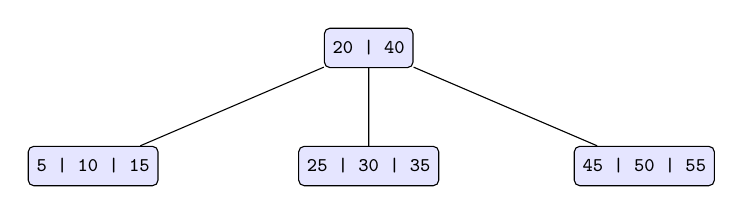
\begin{tikzpicture}[
    >=Stealth,
    bnode/.style={draw, rounded corners=2pt, minimum height=0.5cm,
                  font=\scriptsize\ttfamily, fill=blue!10,
                  inner sep=3pt},
    level 1/.style={sibling distance=3.5cm},
    level 2/.style={sibling distance=1.4cm}
  ]
  \node[bnode] {20 | 40}
    child { node[bnode] {5 | 10 | 15} }
    child { node[bnode] {25 | 30 | 35} }
    child { node[bnode] {45 | 50 | 55} };
\end{tikzpicture}
\end{center}

\vspace{0.5em}
\begin{alertblock}{Design Goal}
A pool-allocated B-Tree with \textbf{no heap}, \textbf{no pointers} (only
\texttt{uint8\_t} node indices), and O($\log n$) operations.
Node size matches FRAM write granularity for NVM-aware storage.
\end{alertblock}
\end{column}
\end{columns}
\end{frame}

% ===========================================================================
\section{B-Tree Theory}
% ===========================================================================

\begin{frame}{B-Tree Properties}
\begin{columns}[T]
\begin{column}{0.48\textwidth}
\textbf{Definition (order $t$):}
\begin{itemize}
  \item Every node has at most $2t - 1$ keys
  \item Every non-root node has at least $t - 1$ keys
  \item Root has at least 1 key (if non-empty)
  \item All leaves are at the same depth
  \item Internal node with $k$ keys has $k + 1$ children
\end{itemize}

\vspace{0.5em}
\textbf{Our configuration ($t = 3$):}
\begin{itemize}
  \item Max keys per node: $2 \times 3 - 1 = 5$
  \item Min keys (non-root): $3 - 1 = 2$
  \item Max children: $2 \times 3 = 6$
  \item Node pool: 15 nodes
\end{itemize}

\vspace{0.5em}
\textbf{Complexity:}
\begin{itemize}
  \item Search: O($\log_t n$)
  \item Insert: O($\log_t n$)
  \item Height: O($\log_t n$)
\end{itemize}
\end{column}

\begin{column}{0.48\textwidth}
\begin{center}
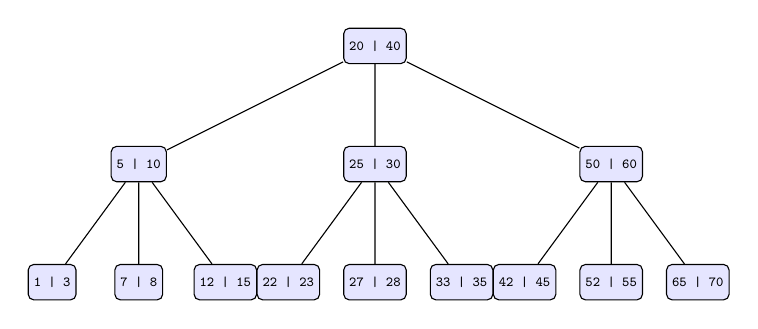
\begin{tikzpicture}[
    >=Stealth,
    bnode/.style={draw, rounded corners=2pt, minimum height=0.45cm,
                  font=\tiny\ttfamily, fill=blue!10, inner sep=2pt},
    level 1/.style={sibling distance=3cm},
    level 2/.style={sibling distance=1.1cm}
  ]
  \node[bnode] (root) {20 | 40}
    child { node[bnode] {5 | 10}
      child { node[bnode] {1 | 3} }
      child { node[bnode] {7 | 8} }
      child { node[bnode] {12 | 15} }
    }
    child { node[bnode] {25 | 30}
      child { node[bnode] {22 | 23} }
      child { node[bnode] {27 | 28} }
      child { node[bnode] {33 | 35} }
    }
    child { node[bnode] {50 | 60}
      child { node[bnode] {42 | 45} }
      child { node[bnode] {52 | 55} }
      child { node[bnode] {65 | 70} }
    };
\end{tikzpicture}
\end{center}

\vspace{0.3em}
\begin{block}{Balance Guarantee}
All leaves at the same depth --- guaranteed.
No rotations needed. Splits propagate upward
only when a node is full.
\end{block}
\end{column}
\end{columns}
\end{frame}

% ---------------------------------------------------------------------------
\begin{frame}{Search Algorithm}
\begin{columns}[T]
\begin{column}{0.48\textwidth}
\textbf{B-Tree search:}
\begin{enumerate}
  \item Start at root node
  \item Linear scan keys in current node
  \item If key found: return success
  \item If node is a leaf: key not in tree
  \item Otherwise: descend to appropriate child
  \item Repeat from step 2
\end{enumerate}

\vspace{0.5em}
\textbf{Example: Search for 27}
\begin{enumerate}
  \item Root: $[20, 40]$ --- $20 < 27 < 40$, go to child 1
  \item Child 1: $[25, 30]$ --- $25 < 27 < 30$, go to child 1
  \item Child: $[27, 28]$ --- found 27 at position 0
\end{enumerate}
\end{column}

\begin{column}{0.48\textwidth}
\begin{center}
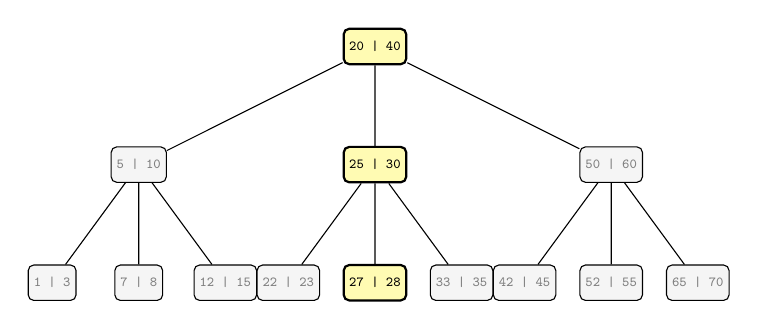
\begin{tikzpicture}[
    >=Stealth,
    bnode/.style={draw, rounded corners=2pt, minimum height=0.45cm,
                  font=\tiny\ttfamily, inner sep=2pt},
    highlight/.style={bnode, fill=yellow!30, thick},
    dim/.style={bnode, fill=gray!8, text=gray},
    level 1/.style={sibling distance=3cm},
    level 2/.style={sibling distance=1.1cm}
  ]
  \node[highlight] (root) {20 | 40}
    child { node[dim] {5 | 10}
      child { node[dim] {1 | 3} }
      child { node[dim] {7 | 8} }
      child { node[dim] {12 | 15} }
    }
    child { node[highlight] {25 | 30}
      child { node[dim] {22 | 23} }
      child { node[highlight] {27 | 28} }
      child { node[dim] {33 | 35} }
    }
    child { node[dim] {50 | 60}
      child { node[dim] {42 | 45} }
      child { node[dim] {52 | 55} }
      child { node[dim] {65 | 70} }
    };
\end{tikzpicture}
\end{center}

\vspace{0.3em}
\begin{block}{Search Path}
Only 3 nodes visited out of 13 total.
$\log_3 n$ levels means far fewer FRAM reads
than a binary tree.
\end{block}
\end{column}
\end{columns}
\end{frame}

% ===========================================================================
\section{Data Structure}
% ===========================================================================

\begin{frame}[fragile]{The \texttt{tiku\_kits\_ds\_btree} Structures}
\begin{columns}[T]
\begin{column}{0.48\textwidth}
\begin{lstlisting}[style=cstyle,
  title={Node and tree structures}]
struct tiku_kits_ds_btree_node {
    tiku_kits_ds_elem_t
        keys[TIKU_KITS_DS_BTREE_MAX_KEYS];
    uint8_t
        children[TIKU_KITS_DS_BTREE_MAX_CHILDREN];
    uint8_t n_keys;
    uint8_t is_leaf;
};

struct tiku_kits_ds_btree {
    struct tiku_kits_ds_btree_node
        nodes[TIKU_KITS_DS_BTREE_MAX_NODES];
    uint8_t root;
    uint8_t n_nodes;
    uint8_t next_free;
};
\end{lstlisting}

\textbf{Memory footprint:}\\
Node: $5 \times 4 + 6 + 2 = 28$ bytes.\\
Tree: $15 \times 28 + 3 = 423$ bytes.
\end{column}

\begin{column}{0.48\textwidth}
\begin{lstlisting}[style=cstyle,
  title={Configuration macros}]
/* Minimum degree (t) */
#define TIKU_KITS_DS_BTREE_ORDER  3

/* Derived constants */
#define TIKU_KITS_DS_BTREE_MAX_KEYS \
    (2 * TIKU_KITS_DS_BTREE_ORDER - 1)  /* 5 */
#define TIKU_KITS_DS_BTREE_MAX_CHILDREN \
    (2 * TIKU_KITS_DS_BTREE_ORDER)      /* 6 */

/* Node pool size */
#ifndef TIKU_KITS_DS_BTREE_MAX_NODES
#define TIKU_KITS_DS_BTREE_MAX_NODES 15
#endif

/* Sentinel: no child / no node */
#define TIKU_KITS_DS_BTREE_NONE  0xFF
\end{lstlisting}

\begin{block}{Pool Allocation}
Nodes are allocated sequentially from
\texttt{nodes[]} via \texttt{next\_free}. No heap,
no free-list --- just bump allocation.
\end{block}
\end{column}
\end{columns}
\end{frame}

% ---------------------------------------------------------------------------
\begin{frame}{Node Layout in Memory}
\begin{center}
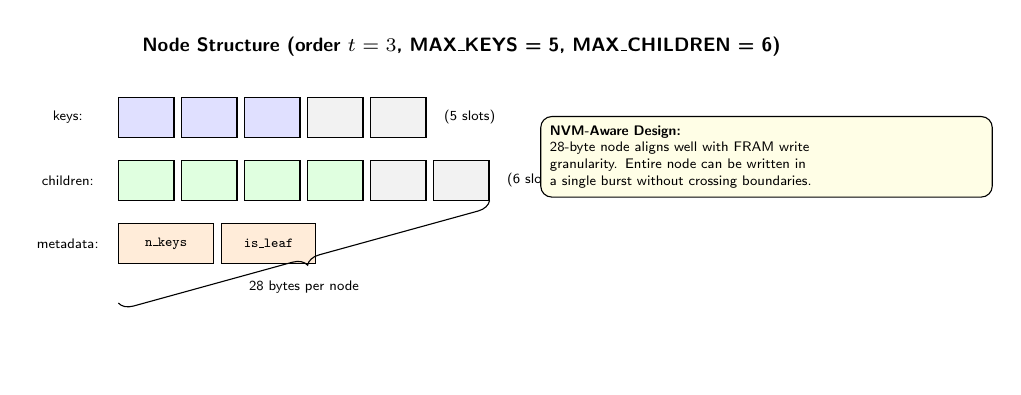
\begin{tikzpicture}[
    cell/.style={draw, minimum width=0.7cm, minimum height=0.5cm,
                 font=\tiny\ttfamily},
    lbl/.style={font=\tiny\sffamily},
    >=Stealth
  ]
  \node[font=\scriptsize\sffamily\bfseries] at (4.5, 3.2)
    {Node Structure (order $t = 3$, MAX\_KEYS = 5, MAX\_CHILDREN = 6)};

  % Keys
  \node[lbl] at (-0.5, 2.3) {keys:};
  \foreach \i in {0,...,4} {
    \pgfmathsetmacro{\fillcol}{\i < 3 ? "blue!12" : "gray!10"}
    \node[cell, fill=\fillcol] (k\i) at (\i*0.8 + 0.5, 2.3) {};
  }
  \node[lbl, right=0.1cm of k4] {(5 slots)};

  % Children (uint8_t indices)
  \node[lbl] at (-0.5, 1.5) {children:};
  \foreach \i in {0,...,5} {
    \pgfmathsetmacro{\fillcol}{\i < 4 ? "green!12" : "gray!10"}
    \node[cell, fill=\fillcol] (c\i) at (\i*0.8 + 0.5, 1.5) {};
  }
  \node[lbl, right=0.1cm of c5] {(6 slots, uint8\_t indices)};

  % n_keys + is_leaf
  \node[lbl] at (-0.5, 0.7) {metadata:};
  \node[cell, fill=orange!15, minimum width=1.2cm] (nk) at (0.75, 0.7) {n\_keys};
  \node[cell, fill=orange!15, minimum width=1.2cm] (il) at (2.05, 0.7) {is\_leaf};

  % Total size
  \draw[decorate, decoration={brace, mirror, amplitude=5pt}]
    (k0.south west) ++(0,-2.1) -- (c5.south east) ++(0,-2.1)
    node[midway, below=7pt, font=\tiny\sffamily] {28 bytes per node};

  % FRAM alignment note
  \node[draw, rounded corners, fill=yellow!10, font=\tiny\sffamily,
        text width=5.5cm, anchor=west] at (5.5, 1.8)
    {\textbf{NVM-Aware Design:}\\
     28-byte node aligns well with FRAM write\\
     granularity. Entire node can be written in\\
     a single burst without crossing boundaries.};
\end{tikzpicture}
\end{center}

\vspace{0.3em}
\begin{columns}[T]
\begin{column}{0.48\textwidth}
\begin{block}{Index-Based Children}
Children are \texttt{uint8\_t} indices into the \texttt{nodes[]} pool ---
not pointers. This makes the tree position-independent and safe
for FRAM persistence.
\end{block}
\end{column}
\begin{column}{0.48\textwidth}
\begin{block}{NONE Sentinel}
\texttt{TIKU\_KITS\_DS\_BTREE\_NONE = 0xFF} marks empty child
slots and indicates ``no node.'' This avoids NULL pointer
issues entirely.
\end{block}
\end{column}
\end{columns}
\end{frame}

% ===========================================================================
\section{API Reference}
% ===========================================================================

\begin{frame}[fragile]{Complete API}
\begin{table}
\centering
\small
\begin{tabular}{@{}lp{8cm}@{}}
\toprule
\textbf{Function} & \textbf{Description} \\
\midrule
\texttt{tiku\_kits\_ds\_btree\_init(bt)}
  & Initialize tree: empty root, reset node pool \\
\texttt{tiku\_kits\_ds\_btree\_insert(bt, key)}
  & Insert key; splits root if full \\
\texttt{tiku\_kits\_ds\_btree\_search(bt, key)}
  & Return 1 if key exists, 0 otherwise \\
\midrule
\texttt{tiku\_kits\_ds\_btree\_min(bt, \&out)}
  & Return smallest key (leftmost leaf, first key) \\
\texttt{tiku\_kits\_ds\_btree\_max(bt, \&out)}
  & Return largest key (rightmost leaf, last key) \\
\texttt{tiku\_kits\_ds\_btree\_count(bt)}
  & Return total number of keys across all nodes \\
\texttt{tiku\_kits\_ds\_btree\_height(bt)}
  & Return tree height (root = 1) \\
\midrule
\texttt{tiku\_kits\_ds\_btree\_clear(bt)}
  & Reset tree to empty state \\
\bottomrule
\end{tabular}
\end{table}

\vspace{0.3em}
\begin{columns}[T]
\begin{column}{0.48\textwidth}
\begin{alertblock}{No Delete Operation}
Delete is intentionally omitted. On embedded systems, B-trees
typically serve as append-only indexes. Clearing the entire
tree and rebuilding is simpler and safer.
\end{alertblock}
\end{column}
\begin{column}{0.48\textwidth}
\begin{block}{Return Codes}
Shared with all DS modules:
\texttt{TIKU\_KITS\_DS\_OK},
\texttt{ERR\_NULL},
\texttt{ERR\_FULL},
\texttt{ERR\_EMPTY},
\texttt{ERR\_NOT\_FOUND}.
\end{block}
\end{column}
\end{columns}
\end{frame}

% ===========================================================================
\section{Insert Algorithm}
% ===========================================================================

\begin{frame}{Insert: Root Splitting}
\begin{columns}[T]
\begin{column}{0.48\textwidth}
\textbf{Insert high-level strategy:}
\begin{enumerate}
  \item If root is full ($n\_keys = 2t-1 = 5$):
  \begin{itemize}
    \item Allocate a new root node
    \item Old root becomes child of new root
    \item Split old root via \texttt{split\_child()}
  \end{itemize}
  \item Call \texttt{insert\_nonfull()} on the (now non-full) root
\end{enumerate}

\vspace{0.5em}
\textbf{Why split at the root?}\\
This is the \emph{only} way a B-tree grows taller.
The tree grows upward from the root, maintaining
the invariant that all leaves are at the same depth.
\end{column}

\begin{column}{0.48\textwidth}
\begin{center}
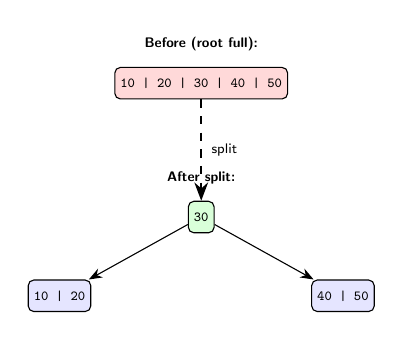
\begin{tikzpicture}[
    >=Stealth,
    bnode/.style={draw, rounded corners=2pt, minimum height=0.4cm,
                  font=\tiny\ttfamily, inner sep=2pt},
    steplbl/.style={font=\tiny\sffamily}
  ]
  % Before: full root
  \node[steplbl, font=\tiny\sffamily\bfseries] at (1.5, 3.5) {Before (root full):};
  \node[bnode, fill=red!15] (r0) at (1.5, 3.0) {10 | 20 | 30 | 40 | 50};

  % After: new root with two children
  \node[steplbl, font=\tiny\sffamily\bfseries] at (1.5, 1.8) {After split:};
  \node[bnode, fill=green!15] (nr) at (1.5, 1.3) {30};
  \node[bnode, fill=blue!10] (nl) at (-0.3, 0.3) {10 | 20};
  \node[bnode, fill=blue!10] (nrr) at (3.3, 0.3) {40 | 50};

  \draw[->] (nr) -- (nl);
  \draw[->] (nr) -- (nrr);

  % Arrow between before/after
  \draw[->, thick, dashed] (r0.south) -- (nr.north)
    node[midway, right, font=\tiny\sffamily] {split};
\end{tikzpicture}
\end{center}

\vspace{0.3em}
\begin{block}{Median Promotion}
The median key (index $t-1$) is promoted to the parent.
Left half stays in the original node, right half moves
to a new node.
\end{block}
\end{column}
\end{columns}
\end{frame}

% ---------------------------------------------------------------------------
\begin{frame}[fragile]{Insert: split\_child and insert\_nonfull}
\begin{columns}[T]
\begin{column}{0.50\textwidth}
\begin{lstlisting}[style=cstyle, basicstyle=\ttfamily\tiny,
  title={split\_child: split a full child node}]
static void split_child(
    struct tiku_kits_ds_btree *bt,
    uint8_t parent_idx,
    uint8_t child_pos)
{
    uint8_t full = bt->nodes[parent_idx]
                       .children[child_pos];
    uint8_t z = bt->next_free++;
    bt->n_nodes++;
    bt->nodes[z].is_leaf =
        bt->nodes[full].is_leaf;
    bt->nodes[z].n_keys = ORDER - 1;

    /* Copy upper half of keys to z */
    for (uint8_t j = 0; j < ORDER - 1; j++)
        bt->nodes[z].keys[j] =
            bt->nodes[full].keys[j + ORDER];

    /* Copy upper half of children to z */
    if (!bt->nodes[full].is_leaf) {
        for (uint8_t j = 0; j < ORDER; j++)
            bt->nodes[z].children[j] =
                bt->nodes[full].children[j+ORDER];
    }

    bt->nodes[full].n_keys = ORDER - 1;

    /* Insert z into parent's children */
    /* Promote median key to parent  */
    /* (shift keys/children right)   */
}
\end{lstlisting}
\end{column}

\begin{column}{0.46\textwidth}
\begin{lstlisting}[style=cstyle, basicstyle=\ttfamily\tiny,
  title={insert\_nonfull: insert into non-full node}]
static void insert_nonfull(
    struct tiku_kits_ds_btree *bt,
    uint8_t node_idx,
    tiku_kits_ds_elem_t key)
{
    int i = bt->nodes[node_idx].n_keys - 1;

    if (bt->nodes[node_idx].is_leaf) {
        /* Shift keys right, insert key */
        while (i >= 0 &&
               bt->nodes[node_idx].keys[i] > key){
            bt->nodes[node_idx].keys[i+1] =
                bt->nodes[node_idx].keys[i];
            i--;
        }
        bt->nodes[node_idx].keys[i+1] = key;
        bt->nodes[node_idx].n_keys++;
    } else {
        /* Find child to descend into */
        while (i >= 0 &&
               bt->nodes[node_idx].keys[i] > key)
            i--;
        i++;
        /* Split child if full */
        if (bt->nodes[
                bt->nodes[node_idx].children[i]
            ].n_keys == MAX_KEYS)
        {
            split_child(bt, node_idx, i);
            if (key > bt->nodes[node_idx].keys[i])
                i++;
        }
        insert_nonfull(bt,
            bt->nodes[node_idx].children[i], key);
    }
}
\end{lstlisting}
\end{column}
\end{columns}
\end{frame}

% ---------------------------------------------------------------------------
\begin{frame}{Insert Walk-Through}
\begin{center}
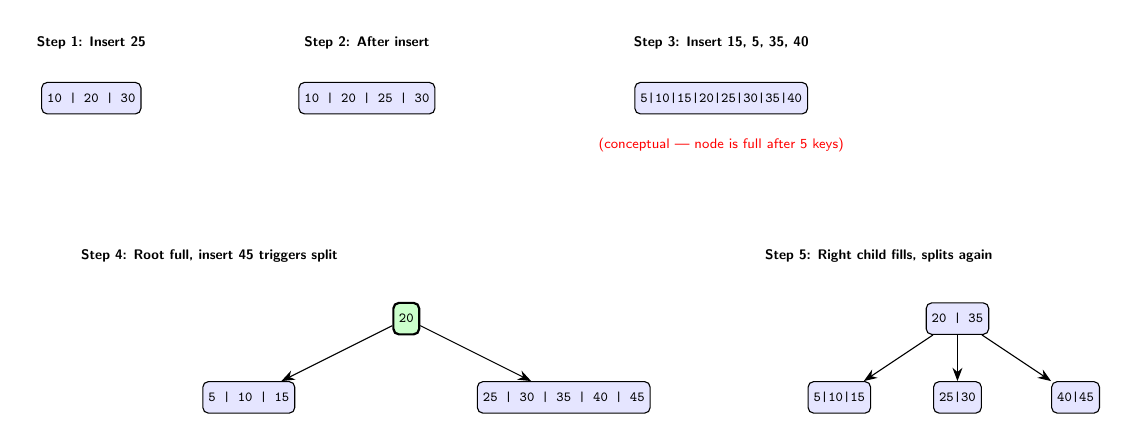
\begin{tikzpicture}[
    >=Stealth,
    bnode/.style={draw, rounded corners=2pt, minimum height=0.4cm,
                  font=\tiny\ttfamily, inner sep=2pt, fill=blue!10},
    highlight/.style={bnode, fill=yellow!30, thick},
    new/.style={bnode, fill=green!20, thick},
    steplbl/.style={font=\tiny\sffamily\bfseries},
    level 1/.style={sibling distance=2.5cm},
    level 2/.style={sibling distance=1.2cm}
  ]
  % Step 1
  \node[steplbl] at (-5, 2.5) {Step 1: Insert 25};
  \node[bnode] at (-5, 1.8) {10 | 20 | 30};

  % Step 2
  \node[steplbl] at (-1.5, 2.5) {Step 2: After insert};
  \node[bnode] at (-1.5, 1.8) {10 | 20 | 25 | 30};

  % Step 3
  \node[steplbl] at (3, 2.5) {Step 3: Insert 15, 5, 35, 40};
  \node[bnode] at (3, 1.8) {5|10|15|20|25|30|35|40};
  \node[font=\tiny\sffamily, text=red] at (3, 1.2) {(conceptual --- node is full after 5 keys)};

  % Step 4: split happens
  \node[steplbl] at (-3.5, -0.2) {Step 4: Root full, insert 45 triggers split};

  \node[new] (nr) at (-1, -1.0) {20};
  \node[bnode] (nl) at (-3, -2.0) {5 | 10 | 15};
  \node[bnode] (nrr) at (1, -2.0) {25 | 30 | 35 | 40 | 45};

  \draw[->] (nr) -- (nl);
  \draw[->] (nr) -- (nrr);

  % Step 5: further inserts
  \node[steplbl] at (5, -0.2) {Step 5: Right child fills, splits again};

  \node[bnode] (nr2) at (6, -1.0) {20 | 35};
  \node[bnode] (nl2) at (4.5, -2.0) {5|10|15};
  \node[bnode] (nm2) at (6, -2.0) {25|30};
  \node[bnode] (nrr2) at (7.5, -2.0) {40|45};

  \draw[->] (nr2) -- (nl2);
  \draw[->] (nr2) -- (nm2);
  \draw[->] (nr2) -- (nrr2);
\end{tikzpicture}
\end{center}

\vspace{0.3em}
\begin{block}{Key Insight: Proactive Splitting}
The CLRS-style B-tree splits full nodes \textbf{on the way down} during insert.
This guarantees we never need to backtrack upward --- a single top-down pass suffices.
\end{block}
\end{frame}

% ===========================================================================
\section{Examples}
% ===========================================================================

\begin{frame}[fragile]{Example 1: FRAM Key Store}
\begin{lstlisting}[style=cstyle,
  title={examples/example\_ds\_btree.c --- persistent key store}]
/* Place B-tree in FRAM for persistence across reboots */
#pragma PERSISTENT(config_index)
struct tiku_kits_ds_btree config_index = {0};

void system_init(void)
{
    /* First boot: initialize the index */
    if (config_index.n_nodes == 0) {
        tiku_kits_ds_btree_init(&config_index);

        /* Store configuration key IDs */
        tiku_kits_ds_btree_insert(&config_index, 0x0001);  /* baud rate */
        tiku_kits_ds_btree_insert(&config_index, 0x0010);  /* sample interval */
        tiku_kits_ds_btree_insert(&config_index, 0x0020);  /* alarm threshold */
        tiku_kits_ds_btree_insert(&config_index, 0x0030);  /* device ID */
        tiku_kits_ds_btree_insert(&config_index, 0x0100);  /* calibration offset */
    }
    /* Subsequent boots: data survives in FRAM */
}

void lookup_config(uint16_t key_id)
{
    if (tiku_kits_ds_btree_search(&config_index, key_id)) {
        /* Key exists in index --- read associated FRAM region */
        load_config_value(key_id);
    }
}
\end{lstlisting}
\end{frame}

% ---------------------------------------------------------------------------
\begin{frame}[fragile]{Example 2: Sorted Sensor Log Index}
\begin{columns}[T]
\begin{column}{0.52\textwidth}
\begin{lstlisting}[style=cstyle,
  title={Building a sorted index of timestamps}]
struct tiku_kits_ds_btree ts_index;
tiku_kits_ds_elem_t min_ts, max_ts;

tiku_kits_ds_btree_init(&ts_index);

/* Log sensor readings with timestamps */
for (uint8_t i = 0; i < n_readings; i++) {
    uint32_t ts = get_timestamp();
    store_reading(ts, readings[i]);
    tiku_kits_ds_btree_insert(
        &ts_index, (tiku_kits_ds_elem_t)ts);
}

/* Query: earliest and latest readings */
tiku_kits_ds_btree_min(&ts_index, &min_ts);
tiku_kits_ds_btree_max(&ts_index, &max_ts);

/* How many readings stored? */
uint8_t total =
    tiku_kits_ds_btree_count(&ts_index);

/* Tree depth (for performance analysis) */
uint8_t h =
    tiku_kits_ds_btree_height(&ts_index);
\end{lstlisting}
\end{column}

\begin{column}{0.44\textwidth}
\begin{center}
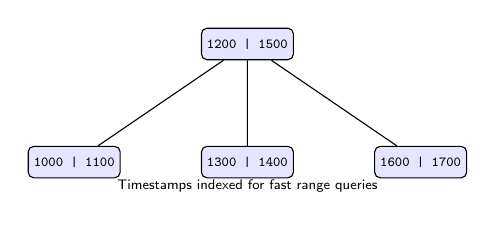
\begin{tikzpicture}[
    >=Stealth,
    bnode/.style={draw, rounded corners=2pt, minimum height=0.4cm,
                  font=\tiny\ttfamily, fill=blue!10, inner sep=2pt},
    level 1/.style={sibling distance=2.2cm}
  ]
  \node[bnode] {1200 | 1500}
    child { node[bnode] {1000 | 1100} }
    child { node[bnode] {1300 | 1400} }
    child { node[bnode] {1600 | 1700} };

  \node[font=\tiny\sffamily] at (0, -1.8)
    {Timestamps indexed for fast range queries};
\end{tikzpicture}
\end{center}

\vspace{0.5em}
\begin{block}{Min/Max Traversal}
\texttt{min()} follows leftmost children to the leftmost leaf.
\texttt{max()} follows rightmost children to the rightmost leaf.
Both are O($\log_t n$).
\end{block}

\vspace{0.3em}
\begin{alertblock}{Range Checking}
With min/max you can quickly determine if a value
falls within the indexed range without a full search.
\end{alertblock}
\end{column}
\end{columns}
\end{frame}

% ===========================================================================
\section{Pool Allocation}
% ===========================================================================

\begin{frame}{Node Pool Allocation}
\begin{columns}[T]
\begin{column}{0.48\textwidth}
\textbf{How node allocation works:}
\begin{enumerate}
  \item \texttt{nodes[]} is a static array of 15 nodes
  \item \texttt{next\_free} starts at 0
  \item Each allocation returns \texttt{nodes[next\_free++]}
  \item No deallocation (no free-list)
  \item \texttt{clear()} resets \texttt{next\_free} to 0
\end{enumerate}

\vspace{0.5em}
\begin{block}{Capacity Planning}
With 15 nodes (order $t=3$), the maximum number of keys is:
\begin{itemize}
  \item Best case (all full): $15 \times 5 = 75$ keys
  \item Worst case (all minimal): $15 \times 2 = 30$ keys
  \item Practical: 40--60 keys depending on insertion order
\end{itemize}
\end{block}
\end{column}

\begin{column}{0.48\textwidth}
\begin{center}
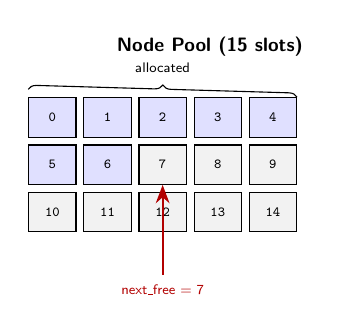
\begin{tikzpicture}[
    cell/.style={draw, minimum width=0.6cm, minimum height=0.5cm,
                 font=\tiny\ttfamily},
    >=Stealth
  ]
  \node[font=\scriptsize\sffamily\bfseries] at (2, 3.2)
    {Node Pool (15 slots)};

  \foreach \i in {0,...,14} {
    \pgfmathsetmacro{\xpos}{mod(\i,5)*0.7}
    \pgfmathsetmacro{\ypos}{2.3 - floor(\i/5)*0.6}
    \pgfmathsetmacro{\fillcol}{\i < 7 ? "blue!12" : "gray!10"}
    \node[cell, fill=\fillcol] (n\i) at (\xpos, \ypos) {\i};
  }

  % next_free arrow
  \draw[->, thick, red!70!black] (1.4, 0.3) -- (n7.south)
    node[pos=0, below, font=\tiny\sffamily] {next\_free = 7};

  % Brace for allocated
  \draw[decorate, decoration={brace, amplitude=3pt}]
    (n0.north west) ++(0, 0.1) -- (n4.north east) ++(0, 0.1)
    node[midway, above=4pt, font=\tiny\sffamily] {allocated};
\end{tikzpicture}
\end{center}

\vspace{0.3em}
\begin{alertblock}{No Fragmentation}
Sequential allocation means zero fragmentation.
When the pool is full, \texttt{insert()} returns
\texttt{ERR\_FULL}. To reclaim space, \texttt{clear()}
and rebuild the tree.
\end{alertblock}
\end{column}
\end{columns}
\end{frame}

% ===========================================================================
\section{NVM Considerations}
% ===========================================================================

\begin{frame}{FRAM and NVM-Aware Design}
\begin{columns}[T]
\begin{column}{0.48\textwidth}
\begin{block}{Why FRAM-Friendly?}
\begin{itemize}
  \item \textbf{No pointers}: indices survive relocation
  \item \textbf{Contiguous nodes}: each node is 28 bytes,
        written as a single FRAM burst
  \item \textbf{Power-fail safe}: partial writes corrupt
        at most one node
  \item \textbf{Persistent pool}: \texttt{\_\_persistent} attribute
        keeps tree across reboots
\end{itemize}
\end{block}

\begin{block}{MSP430FR5969 FRAM Layout}
\begin{itemize}
  \item 64\,KB FRAM total
  \item B-tree uses 423 bytes ($< 1\%$)
  \item Remaining FRAM for data storage
  \item Tree serves as index into data regions
\end{itemize}
\end{block}
\end{column}

\begin{column}{0.48\textwidth}
\begin{center}
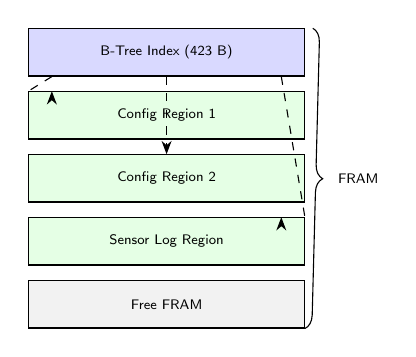
\begin{tikzpicture}[
    box/.style={draw, minimum width=3.5cm, minimum height=0.6cm,
                font=\tiny\sffamily, text centered},
    >=Stealth
  ]
  \node[box, fill=blue!15] (btree) at (0, 3.0) {B-Tree Index (423 B)};
  \node[box, fill=green!10] (data1) at (0, 2.2) {Config Region 1};
  \node[box, fill=green!10] (data2) at (0, 1.4) {Config Region 2};
  \node[box, fill=green!10] (data3) at (0, 0.6) {Sensor Log Region};
  \node[box, fill=gray!10] (free) at (0, -0.2) {Free FRAM};

  \draw[decorate, decoration={brace, amplitude=5pt}]
    (btree.north east) ++(0.1, 0) -- (free.south east) ++(0.1, 0)
    node[midway, right=7pt, font=\tiny\sffamily] {FRAM};

  \draw[->, dashed] (btree.south west) ++(0.3,0) -- (data1.north west) ++(0.3,0);
  \draw[->, dashed] (btree.south) -- (data2.north);
  \draw[->, dashed] (btree.south east) ++(-0.3,0) -- (data3.north east) ++(-0.3,0);
\end{tikzpicture}
\end{center}

\vspace{0.3em}
\begin{alertblock}{Power-Fail Recovery}
If power fails during a split, at most the new node and
parent are inconsistent. On reboot, detect via
\texttt{n\_nodes} vs.\ \texttt{next\_free} mismatch and
rebuild if needed.
\end{alertblock}
\end{column}
\end{columns}
\end{frame}

% ===========================================================================
\section{Test Suite}
% ===========================================================================

\begin{frame}{Test Cases Overview}
\begin{table}
\centering
\small
\begin{tabular}{@{}clp{7cm}@{}}
\toprule
\textbf{\#} & \textbf{Test Function} & \textbf{What It Verifies} \\
\midrule
1 & \texttt{test\_kits\_ds\_btree\_init}
  & Proper initialization, empty tree \\
2 & \texttt{test\_kits\_ds\_btree\_insert\_search}
  & Insert keys, verify all are searchable \\
3 & \texttt{test\_kits\_ds\_btree\_split}
  & Root split creates new root with correct children \\
4 & \texttt{test\_kits\_ds\_btree\_multi\_split}
  & Multiple splits maintain B-tree invariants \\
5 & \texttt{test\_kits\_ds\_btree\_min\_max}
  & Min/max correct after various insertions \\
6 & \texttt{test\_kits\_ds\_btree\_count}
  & Count matches number of inserted keys \\
7 & \texttt{test\_kits\_ds\_btree\_height}
  & Height grows correctly with splits \\
8 & \texttt{test\_kits\_ds\_btree\_pool\_full}
  & Returns \texttt{ERR\_FULL} when node pool exhausted \\
9 & \texttt{test\_kits\_ds\_btree\_clear}
  & Clear resets all state \\
10 & \texttt{test\_kits\_ds\_btree\_null\_inputs}
  & All functions reject NULL with \texttt{ERR\_NULL} \\
\bottomrule
\end{tabular}
\end{table}
\end{frame}

% ===========================================================================
\section{Complexity Analysis}
% ===========================================================================

\begin{frame}{B-Tree vs.\ Other Structures}
\begin{table}
\centering
\small
\begin{tabular}{@{}lcccc@{}}
\toprule
\textbf{Operation} & \textbf{B-Tree} & \textbf{Sorted Array} & \textbf{Hash Table} & \textbf{BST (unbal.)} \\
\midrule
Search      & O($\log_t n$) & O($\log n$)  & O(1) avg    & O($n$) worst \\
Insert      & O($\log_t n$) & O($n$)       & O(1) avg    & O($n$) worst \\
Min/Max     & O($\log_t n$) & O(1)         & O($n$)      & O($n$) worst \\
Ordered     & Yes           & Yes          & No          & Yes \\
Balanced    & Always        & N/A          & N/A         & No \\
Memory      & 423\,B        & 66\,B        & 128--256\,B & Variable \\
Complexity  & High          & Low          & Medium      & Low \\
\bottomrule
\end{tabular}
\end{table}

\vspace{0.5em}
\begin{columns}[T]
\begin{column}{0.48\textwidth}
\begin{block}{Use B-Tree When\ldots}
\begin{itemize}
  \item You need guaranteed O($\log n$) for all operations
  \item Frequent inserts and lookups
  \item Ordered traversal required
  \item Data persists in FRAM across reboots
\end{itemize}
\end{block}
\end{column}

\begin{column}{0.48\textwidth}
\begin{block}{Use Something Simpler When\ldots}
\begin{itemize}
  \item Fewer than 16 elements $\rightarrow$ sorted array
  \item Only exact-match lookup $\rightarrow$ hash table
  \item Read-heavy, write-rare $\rightarrow$ sorted array
  \item Memory is extremely tight $\rightarrow$ sorted array
\end{itemize}
\end{block}
\end{column}
\end{columns}
\end{frame}

% ===========================================================================
\section{Summary}
% ===========================================================================

\begin{frame}{Summary}
\begin{columns}[T]
\begin{column}{0.48\textwidth}
\begin{block}{What We Built}
\begin{itemize}
  \item Pool-allocated B-tree (no heap)
  \item Order $t = 3$: 2--5 keys per node
  \item \texttt{uint8\_t} index-based children (no pointers)
  \item O($\log_t n$) search and insert
  \item 423 bytes state (15 nodes)
  \item FRAM/NVM-aware node layout
\end{itemize}
\end{block}

\begin{block}{Key Design Choices}
\begin{itemize}
  \item Bump allocation for node pool
  \item \texttt{0xFF} sentinel for empty slots
  \item No delete (clear + rebuild instead)
  \item Proactive splitting on insert
\end{itemize}
\end{block}
\end{column}

\begin{column}{0.48\textwidth}
\begin{block}{Use Cases}
\begin{itemize}
  \item FRAM persistent key store
  \item Sorted sensor log index
  \item Configuration parameter lookup
  \item Range checking for alarm thresholds
\end{itemize}
\end{block}

\begin{block}{Files}
\scriptsize
\begin{tabular}{@{}lp{4.5cm}@{}}
Header: & \texttt{ds/tree/tiku\_kits\_ds\_btree.h} \\
Source: & \texttt{ds/tree/tiku\_kits\_ds\_btree.c} \\
Tests: & \texttt{tests/ds/test\_kits\_ds\_btree.c} \\
Example: & \texttt{examples/example\_ds\_btree.c} \\
\end{tabular}
\end{block}
\end{column}
\end{columns}
\end{frame}

% ---------------------------------------------------------------------------
\begin{frame}{Thank You}
\begin{center}
\Large\textbf{TikuKits DS: B-Tree}\\[0.5em]
\normalsize Balanced Search Trees for Resource-Constrained Endpoints\\[1.5em]

\begin{tabular}{rl}
  Repository: & \url{https://github.com/tikuos/tikuOS} \\
  License:    & Apache 2.0 \\
  Common:     & \texttt{tikukits/ds/tiku\_kits\_ds.h} \\
  Header:     & \texttt{tikukits/ds/tree/tiku\_kits\_ds\_btree.h} \\
  Source:     & \texttt{tikukits/ds/tree/tiku\_kits\_ds\_btree.c} \\
  Tests:      & \texttt{tikukits/tests/ds/test\_kits\_ds\_btree.c} \\
  Examples:   & \texttt{tikukits/examples/example\_ds\_btree.c} \\
\end{tabular}
\end{center}
\end{frame}

\end{document}
